\chapter[Laplace - Borel transform and conjugate diagram...]{Laplace - Borel transform and conjugate diagram
 of an entire function of exponential type}\label{chap9}%chap 9 

\section[Conjugate diagram and Laplace - Borel...]{Conjugate diagram and Laplace - Borel\hfil\break
  transform}\label{chap9:sec1} %sec 1 

We\pageoriginale recall the formulae: $\varphi (z)$ is holomorphic on $C$ and
vanishes at infinity ; $\Phi (w)$ is an entire function of exponential
type $b$. 
\begin{align*}
 \Phi (w) & = \frac{1}{2 \pi i} \int_C e^{wz} \varphi (z) dz
 \tag{1}\label{chap9:sec1:eq1} \\
 \varphi (z) & = \int^\infty_0 \Phi (u) e^{-uz} dz ; Re z >
 b. \tag{2}\label{chap9:sec1:eq2} 
\end{align*}
If (\ref{chap9:sec1:eq1}) and (\ref{chap9:sec1:eq2}) hold, then
\begin{equation*}
 \varphi_o (z) = \varphi (z) \text{ for } Re z >
 b. \tag{3}\label{chap9:sec1:eq3}  
\end{equation*}
$h (\theta) = \lim \sup \dfrac{ \log |\Phi (r e^{i \theta})|}{r}=$ the
type of $\Phi (w)$ in the direction $\theta$. 

Interpretation of (\ref{chap9:sec1:eq1}): 
$$
\Phi (r e^{i \theta}) \le e^{rk_c^{(\theta)}} \times \frac{1}{2 \pi }
\int \varphi (z) dz 
$$
where $k_c (\theta) = \sup\limits_{z \in c} Re (ze^{i \theta})$.

Interpretation of $k_c (\theta)$: the closed convex hull of $C$ is the
intersection of the half planes $x$ cos $\theta - y \sin \theta \le
k_c (\theta)$. Let $k(\theta) = \inf k_c (\theta)$. Then the
intersection of the planes $x \cos \theta - y \sin \le k (\theta)$, 
is the smallest convex set outside of which $\varphi (z)$ is
holomorphic. By abuse of language we call this set ``the convex hull
of the singularities of $\varphi$''. 

Evidently\pageoriginale $h(\theta) \le k_c (\theta)$ and so $h (\theta) \le k (\theta)$.

Interpretation of (2): we consider the following equation
\begin{equation*}
 \varphi_\alpha (z) = \int\limits^{\infty e^{i \alpha}}_0 \Phi (w) e^{-wz}
 dw, w= r e^{i \chi}. \tag{$2_\alpha$} 
\end{equation*}

We have $\varphi_\alpha (z)$ holomorphic for Re $z e^{i \alpha} > h
(\alpha)$. In the same manner we have the equation: 
\begin{equation*}
\varphi_\beta (z) = \int\limits^{\infty e^{i \beta}}_0 \Phi (w) e^{-wz} dw, w = r e^{i \beta} \tag{$2_\beta$}
\end{equation*}

\noindent 
\begin{minipage}[c]{5.8cm}
We have $\varphi_\beta (Z)$ holomorphic for Re $z e^{i \beta} > h
(\beta)$. Suppose $\alpha \nequiv \beta (\mod 2 \pi)$. Then the
intersection of the half-planes in which $\varphi_\alpha$ and
$\varphi_\beta$ are holomorphic is non-empty; moreover for any point
in the intersection of these halfplanes we have $\varphi_\alpha (z) =
\varphi_\beta (z)$. For this it is sufficient to show that $\int_C
\Phi (w) e^{-wz} dw \to 0$ as $R \to \infty$, where $C$ is the smaller are
joining $R e^{i \beta}$ and $R e^{i \alpha}$. Since $w^2 \Phi (w)
e^{-wz}$ is bounded on the lines $(0, \infty e^{i \beta})$ and $(0,
\infty e^{i \alpha})$ it is sufficient to apply the theorem of
Phragmen Lindelof. 
\end{minipage}
\begin{minipage}[c]{5cm}
\begin{figure}[H]
\centerline{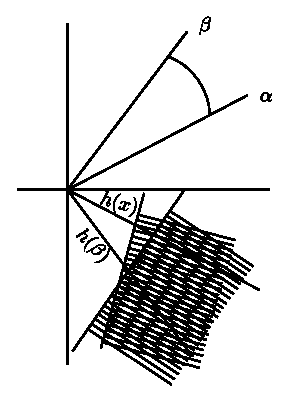
\includegraphics{vol15-figures/fig15-1.eps}}
\end{figure}
\end{minipage}

Thus we have $\varphi (z)$ defined and holomorphic outside of every
half plane $x \cos \alpha - y \sin \alpha \le h (\alpha)$. Hence $k
(\theta) \le h (\theta)$ and we have the following theorem: 
\begin{theorem*}%theo 0
 The\pageoriginale equations
 \begin{align*}
   \Phi (w) &= \frac{1}{2 \pi i} \int_C e^{wz} \varphi (z) dz \tag{1}\\
   \varphi_\alpha (z) & = \int_0^{\infty e^{i \alpha}} \Phi (w) e^{-wz }dz \tag{2}
 \end{align*}
 allow us to associate to each function $\varphi$, holomorphic at
  infinity and vanishing there, an entire function $\Phi$ of
  exponential type and conversely. If $S$ is the ``convex hull of
  the singularities'' of $\varphi (z)$ and $h (\theta)$ the type of
  $\Phi (w)$ in the direction $\theta$, then $S$ is the
  intersection of the half-planes $x \cos \theta - y \sin \theta
  \le h (\theta) (0 \le \theta \le 2 \pi )$. 
\end{theorem*}

\begin{defi*}%defin
 $\varphi(z)$ is defined to be the {\em Laplace-Boral} transform of
 $\Phi (w)$ and $S$ is defined to be the {\em conjugate diagram } of
 $\Phi (w)$. 
\end{defi*}

The notion of the conjugate diagram is due to G. Polya.

\section{Basis and Fourier development in \texorpdfstring{$\mathscr{H}_\Lambda
  (\Omega)$}{mathscrH}}\label{chap9:sec2} %Sec 2

We suppose for simplicity $\Lambda$ to be simple and we consider the
Fourier development of functions in $\mathscr{H}_\Lambda
(\Omega)$. The formal development will be established if we prove that
$\{e^{\lambda z}\}$ form a basis in $\mathscr{H}_\Lambda (\Omega)$. 

\setcounter{theorem}{0}
\begin{theorem}\label{chap9:sec2:thm1}%theo 1
  Suppose $\Omega$ is connected and $\mathscr{H}_\Lambda (\Omega) \neq
  \mathscr{H} (\Omega)$. Then $\{e^{\lambda z}\}_{\lambda \in
    \Lambda}$ form a basis in $\mathscr{H}_\Lambda (\Omega)$. 
\end{theorem}

Since $\mathscr{H}_\Lambda (\Omega) \neq \mathscr{H}(\Omega)$, there
exists a measure $d \mu \in \mathscr{H}' \Omega$ with $\int e^{\lambda
 z} d \mu (z) \neq 0, \lambda \in \Lambda$. Since $\Omega$ is
connected a closed rectifiable cure $C$ can be found with the support
of $d \mu$ in its interior. Then we have the following equations: 
$$
\Phi (w) = \int e^{wz} d \mu (z) = \frac{1}{ 2 \pi i} \int_C e^{wz}
\varphi (z) dz 
$$

We\pageoriginale have trivially, $\bigg\{ e^{\lambda z} \bigg\}_{\lambda \in
 \Lambda}$ total in $\mathscr{H}_\Lambda (\Omega)$. To show that
$\bigg\{ e^{\lambda z} \bigg\}$ is free it is sufficient to show that
there exists a measure which is orthogonal to all $e^{\lambda z}$
except one, say $\lambda_1$. For this it is sufficient to suppose 
that $\lambda_1 = \theta \in \Lambda$. We have $\Phi (0) = 0,
i.e. \int_0 \varphi(z) dz = 0$. Let $\varphi_1$ be the primitive of
$\varphi$ which vanishes at infinity. Since $\int_C \varphi (z) dz =
0$, we have $\Phi (w) = - \dfrac{1}{2 \pi i} w \int_C e^{wz} \varphi_1
(z) dz$. If $\dfrac{\Phi (w)}{w} \neq 0$, we have a measure $d \mu$,
given by $\varphi_1 (z)$ not orthogonal to $i = e^{oz}$. In the
contrary case we iterate the process.
 
\begin{coro*}%colo 0
 If $\Omega' \supset \Omega, \Omega'$ open and $\Omega$ connected and
 if $\mathscr{H}_\Lambda (\Omega) \neq \mathscr{H}(\Omega)$ then
 $\{e^{\lambda z}\}_{\lambda \in \Lambda}$ form a basis of
 $\mathscr{H}_\Lambda (\Omega')$. 
\end{coro*}

\begin{remark}\label{chap9:sec2:rem1}%rema1
 We cannot extend the result to the case where $\Omega$ is not
 connected. For let $\Lambda = Z$ and $\Omega$ consist of two
 disjoint circular domains around $\pi i$ and $- \pi i$. Here $1 \in
 $ span of $\{e^{nz}\} n \neq 0$. 
\end{remark}

\begin{remark}\label{chap9:sec2:rem2}%rema 2
 Let $\Phi (w) = \dfrac{1}{2 \pi i} \int_C e^{wz} \varphi (Z) dz$ and
 $\Phi (\Lambda) = 0$. Then for each $\lambda \in \Lambda$, we can
 find $\varphi_\Lambda (z)$ holomorphic outside the same convex
 domain as $\varphi (z)$ and satisfying the equation 
 $$
 \frac{\Phi (w)}{w - \lambda} = \frac{1}{2 \pi i} \int_C e^{wz}
 \varphi_\lambda (z) dz. 
 $$
\end{remark}


\begin{theorem}\label{chap9:sec2:thm2}%theo 2
 Suppose $\Omega$ is convex and $\mathscr{H}_\Lambda (\Omega)
 \neq \mathscr{H} (\Omega)$. Then every $f \in \mathscr{H}_\Lambda
 (\Omega)$ is uniquely defined by its development. In other words
 if all the coefficients in the development of $f$ are zero, the
 function is identically zero. 
\end{theorem}

\begin{proof}
 Let\pageoriginale $g \in \mathscr{H}_\Lambda (\Omega)$ and $g(z) \sim \sum 0
 e^{\Lambda z}$. Let $\Phi (w)$ and $\varphi (z)$ be determined as
 before with $\Phi (\Lambda) = 0$. We have the equation 
 $$
 \Phi_\lambda (w) = \Phi (w) / (w-\lambda) = \frac{1}{2 \pi i} \int_c
 \varphi_\lambda (z) e^{wz} dz. 
 $$

 By our hypothesis, we have for every $\lambda \in \Lambda, \int_c
 \varphi_\lambda (z) g(z) dz = 0$.
\end{proof}

 Now $\Phi (w) = w^p e^{aw} \prod\limits_{\lambda \in \Lambda} \left(1 -
 \dfrac{w}{\lambda}\right) e^{w/ \lambda}$. 
 $$
 \Phi' (w) = a \Phi + \frac{p \Phi_o (w)}{w} + \sum_\lambda
 \left(\frac{\Phi}{\lambda} + \Phi_\lambda\right). 
 $$

We set $X_\lambda (w) = \Phi (w) / \lambda + \Phi_\lambda (w)$. In the
same way as we have proved in the case of mean periodic functions
(Lecture 5, \S \ref{chap5:sec1}) we have the following inequalities: 
\begin{align*}
 \big|X_\lambda~ (w)\big|~ & < ~\frac{2}{\big|\lambda \big|^2}~
 \big|w~ \Phi~ (w)\big|~ \text{ when }~ \big|w - \lambda \big|~
 >~ \frac{\big|\lambda \big|}{2}\\ 
 \big|X_\lambda~ (w)\big|~ & < ~\frac{2}{\big|\lambda \big|^2}~
 \big|w~ \Phi~ (w)\big|~ \text{ when } 1 \le \big| w - \lambda \big|
 \frac{|\lambda|}{2}\\ 
 \big|X_\lambda~ (w)\big|~ & < ~\frac{K}{\big|\lambda \big|^2}
 \sup\limits_{ |w - w'| = 2 } \big| w^{'2} \Phi (w') \big| \text{
 when } \big|w - \lambda \big| < 1. 
\end{align*}

Therefore we have the following inequality
$$
\big|X_\lambda~ (w)\big|~ < ~\dfrac{K}{\big|\lambda \big|^2}
e^{h (\theta) \big| w \big| + \varepsilon \big| w \big|} 
$$
uniformly in $w$. Since $\Omega$ is convex, we can take a path $C$ in
$\Omega$ around the conjugate diagram of $\Phi$ and by taking the
Laplace-Borel transform along this path we have $\big| \varphi_\lambda
(z) + \varphi (z) / \lambda \big| < K/ \big| \lambda \big|^2$
uniformly in $z$. Therefore we have the following implication: 
$$
\int_c g(z) \left[ a \varphi + p \varphi_o + \sum (\varphi_\lambda +
 \varphi/_\lambda )\right] dz = 0 \Longrightarrow \int_c g(z) z \varphi (z)
dz =0. 
$$

As the same holds if we replace $\varphi (z)$ by $\varphi_\lambda
(z)$, we have $z g (z) \in \mathscr{H}_\Lambda (\Omega)$ and $zg (z)
\sim \sum o e^{\lambda z}$. Therefore if $g (z) \sim \sum oe^{\lambda
 z} \in \mathscr{H}_\Lambda (\Omega) g (z)\break P (z) \in \mathscr{H}_\Lambda
(\Omega)$ for every polynomial $P(z)$. If $g(z) \nequiv 0$. We can
suppose that $g (z)$ has only a finite number of zeros in $\Omega-$ if
necessary we\pageoriginale can replace $\Omega$ by a smaller domain containing $C-$
so that every holomorphic function with these zeros is in
$\mathscr{H}_\Lambda (\Omega)$, and $\mathscr{H}_\Lambda (\Omega) =
\mathscr{H} (\Omega)$, contrary to the hypothesis that
$\mathscr{H}_\Lambda (\Omega) \neq \mathscr{H}(\Omega)$. 

\begin{remark*}%remar 0
 Suppose $\Omega' \subset \Omega, \Omega$ convex and
 $\mathscr{H}_\Lambda (\Omega) \neq \mathscr{H} (\Omega)$. Then one
 cannot assert that every $f \in \mathscr{H}_\Lambda (\Omega')$ is
 determined by its development. As an example, let $\Lambda=$ set of
 integers and $\Omega$ be a convex set containing $\pi i $ and $- \pi
 i$. Let $\Omega_i$ be disjoint from $\Omega$, and contained in $Rez
 > 0, \big| Imz \big| < \pi$. We take $\Omega' = \Omega \cup
 \Omega_1, f = 0$ in $\Omega, f$ analytic $\nequiv 0$ in
 $\Omega_1$.
\medskip

\noindent 
\begin{minipage}[c]{5.8cm} 
 Let us put $Z = e^z, f(z) = F(Z)$. $F$ is zero on the
 set $\log \Omega$; and analytic $\nequiv 0$ in $\log \Omega_1$. By
 the theorem of Runge, $F$ can be approximated by polynomials in
 $\log \Omega_1$, and then $f \in \mathscr{H}_\Lambda (\Omega_1)$. As
 $\{e^{nz}\} n \in N$ is a basis in $\mathscr{H}_\Lambda (\Omega)$,
 the development of $f$ has zero coefficients, what ever be $f$ in
 $\Omega_1$. 
\end{minipage}
\begin{minipage}[c]{5cm}
\begin{figure}[H]
\centerline{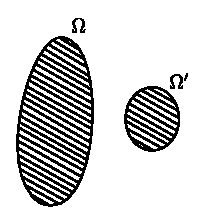
\includegraphics{vol15-figures/fig15-2.eps}}
\end{figure}
\end{minipage}
\end{remark*}

\noindent \textbf{Problems. }
 \begin{enumerate}[1)]
 \item It is possible to get a statement like the above theorem if
 the open convex set $\Omega$ is replaced by a closed convex set? 
 \item Also, is a similar statement possible on replacing the open
 convex set $\Omega$ by an open connected set ? 
 \end{enumerate}
